\documentclass{article}
\usepackage{geometry}[1in]
\usepackage{amsmath}
\usepackage{relsize}
\usepackage{graphicx}
\usepackage{bm}
\author{Taylor Colburn, Kate Hoverson, Mack Baker, Nathaniel Chrisman}
\title{Multi-parameter model fitting to damped harmonic oscillator data: a primer }
\date{\today}
\begin{document}
  \maketitle
  \begin{abstract}
    Displacement of a pendulum with damped harmonic oscillation was measured against time. The obtained data was analyzed against a theoretical model of damped harmonic oscillation, the parameters of which were estimated by the authors. Excel “Solver” was used to minimize root-mean-square (RMS) value of residuals, which resulted in a final value of $7.910 \times 10^{-5}$.
  \end{abstract}
  \section{Introduction}

  The goal of this experiment is to obtain experimental data from a damped harmonic oscillator (pendulum) and to fit a theoretical model with many parameters to the data obtained. In order for the experimental data to be compared completely to the model, a few parameters need to be calculated and/or derived. Some of these parameters can be derived through observation of the data, such as amplitude and decay constant, while others were calculated or minimized, such as angular frequency and phase offset.

  The model of a damped harmonic oscillator is given by the following equation:

  \begin{equation} \label{eq_1}
    y(t) = exp\left(\dfrac{-t}{\tau}\right) A\cos{\left(\omega t - \phi \right)} + \alpha
  \end{equation}

  where,
  $$t = \text{time}$$
	$$\tau  = \text{decay constant}$$
	$$\omega = \text{angular frequency}$$
	$$\phi = \text{phase offset}$$
	$$\alpha = \text{offset of pendulum}$$
	$$y = \text{position}$$
	$$A = \text{amplitude}$$

  Assuming all of these values were estimated with reasonable accuracy, the model ought to represent the motion of a damped harmonic oscillator to within a small degree of error, as signified by the size of residuals at each point.

  \section{Procedure}

  In order to observe a damped simple harmonic oscillator (DSHO), a lightweight foam ball was used as the pendulum so as to cause a rapid decrease in amplitude due to drag. The DSHO was observed with a Vernier motion detector using Graphical Analysis. This collected data was then transported to Excel. The seven values shown in the introduction were either measured or calculated. These values were used with \ref{eq_1} to determine the RMS value between the experimental data and the calculated (model) data. The calculated values above were generated via Excel Solver.

  \section{Results}

  The seven values shown in the introduction are as follows:

  \begin{table}[!h]
    \centering
    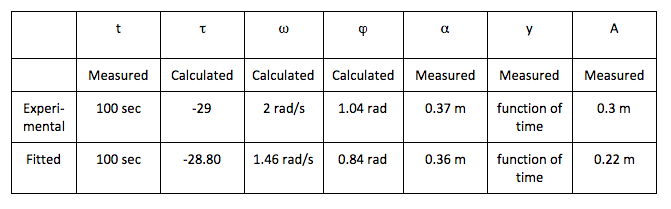
\includegraphics[scale=.6]{table1.png}
    \caption{Recorded and fitted values for the damped oscillator}
    \label{table1}
  \end{table}

  Before Excel Solver was used the RMS value was calculated to be approximately $2.33 \times 10^{-3}$. After Excel Solver was used the RMS value was calculated to be $7.92 \times 10^{-5}$. Residual was calculated from the difference of fitted and experimental values.

  \clearpage

  \begin{figure}[!ht]
    \centering
    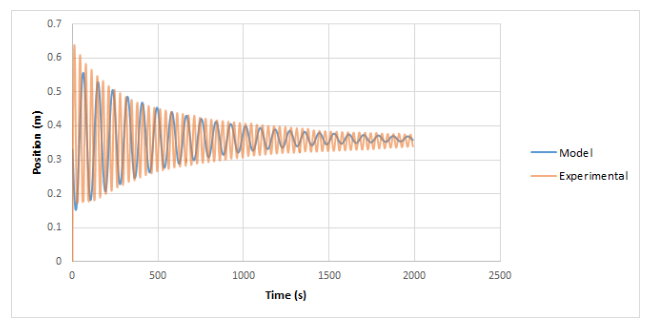
\includegraphics[scale=.65]{Model_vs_experiment.png}
    \caption{Plot showcasing the experimental data against the model data with respect to time and amplitude.}
    \label{mod_v_exp}
  \end{figure}

  \begin{figure}[!h]
    \centering
    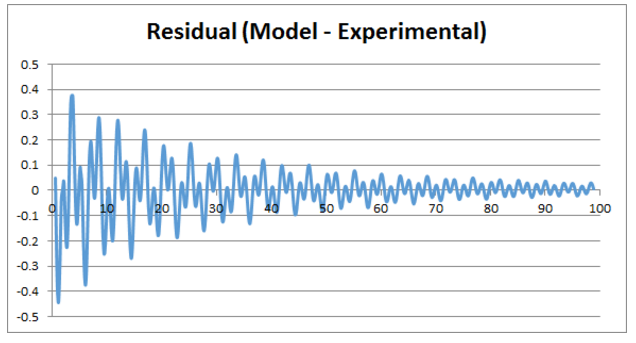
\includegraphics[scale=.6]{Residuals.png}
    \caption{Plot of residuals calculated from the difference of fitted and experimental values.}
    \label{residuals}
  \end{figure}

  \clearpage

  \section{Discussion}

  These results demonstrate the degree of difficulty that comes with multi-parameter model-fitting, particularly when researchers use techniques they don’t have a strong understanding of. While many values optimized in the theoretical model fit trivially close to the experimental values, three parameters deviated substantially: the angular frequency, phase offset, and amplitude (see; table 1). The largest discrepancies can be seen between the two values of both angular frequency and amplitude, where model values were $73.0\%$ and $73.3\%$ of experimental values, respectively. The model phase offset, while less dramatic, still constituted approximately $80.8\%$ of the measured figure.

  These deltas between empirically-gathered and model-derived quantities were almost certainly due to difficulties applying Excel’s Solver plug-in, in combination with what errors arose from manually modifying post-hoc. The majority of time during data analysis was spent attempting to minimize the residuals using an improper algorithm for the shape and character of the data, to no avail. In the final moments of said analysis, the proper algorithm was chosen, and a fit was applied that, indeed, minimized the residuals by two orders of magnitude. However, the plotted results of this process showed gross disagreement between the two. The model data were subsequently shifted vertically to fit more closely to the recorded findings. Figure 2 clearly demonstrates that, while the RMS residual value was notably tiny, local residual values were nearly the magnitude of the data itself.

  \section{Conclusion}

  Despite care taken on the part of the authors, a lack of experience and knowledge of the tools employed --- as well as the inherent difficulty of model-fitting in relatively high dimensional parameter spaces --- resulted in a bad fit. In future investigations, the authors advise the use of more flexible fitting algorithms, as opposed to the default plug-ins available to popular software programs such as Excel. In addition, the RMSR appears to be a poor metric to determine the goodness-of-fit of a theoretical model.

  \clearpage

  \section{Appendix}

    \begin{figure}[!ht]
      \centering
      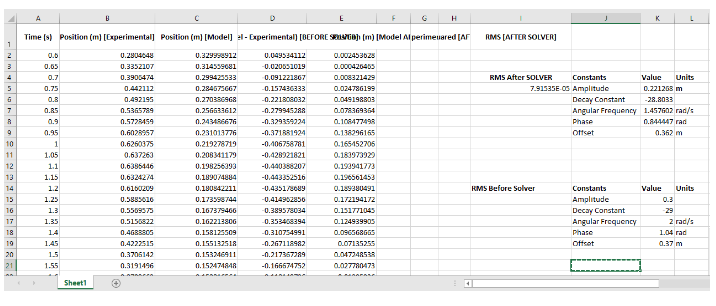
\includegraphics[scale=.6]{raw_data.png}
      \caption{Page 1 of raw data. Column D shows residuals before fitting with Excel Solver. These residuals were calculate by the difference of fitted parameters and experimental results: $R = d_p - d_f,$ where  R is residual, $d_p$ is the actual displacement of the pendulum and $d_f$ is the displacement predicted by the model. The square root of the average of these residual values were used to manually calculate the RMS before using solver: $\text{RMSR} = \sqrt{\frac{1}{N} \sum\limits_{i=1}^N R_i},$ where $R_i$ is the ith residual, and $N$ is the total number of data points.}
      \label{raw}
    \end{figure}

\end{document}
